% Experiments chapter for ZK-DAC (party B). Standalone: % generated by make_numbers.py — do not edit; every value is listed with its source in CLAIM_LEDGER.md
\newcommand{\NConsVnineA}{60,622}
\newcommand{\NConsVnineB}{105,424}
\newcommand{\NConsVnineC}{150,226}
\newcommand{\NConsVnineD}{195,028}
\newcommand{\NConsTransfer}{84,008}
\newcommand{\NConsReg}{17,436}
\newcommand{\NConsRevoke}{51,815}
\newcommand{\NPubVnineD}{20}
\newcommand{\NPubVeightD}{27}
\newcommand{\NGasVnineFreshD}{564,147}
\newcommand{\NMutFieldA}{199}
\newcommand{\NMutSemA}{37}
\newcommand{\NMutUnexpA}{0}
\newcommand{\NMutFieldB}{282}
\newcommand{\NMutSemB}{49}
\newcommand{\NMutUnexpB}{0}
\newcommand{\NMutFieldC}{408}
\newcommand{\NMutSemC}{62}
\newcommand{\NMutUnexpC}{0}
\newcommand{\NMutFieldD}{534}
\newcommand{\NMutSemD}{76}
\newcommand{\NMutUnexpD}{0}
\newcommand{\NTthreeRows}{170}
\newcommand{\NTthreeAgRej}{114}
\newcommand{\NTthreeAgAcc}{28}
\newcommand{\NTthreeBwo}{7}
\newcommand{\NTthreeFa}{21}
\newcommand{\NTthreeFaPolicy}{20}
\newcommand{\NTthreeGap}{0}
\newcommand{\NExTotal}{534}
\newcommand{\NExStmt}{3}
\newcommand{\NEtwoVsevenAcc}{640}
\newcommand{\NEtwoVsevenSub}{64}
\newcommand{\NEtwoVeightAcc}{100}
\newcommand{\NEtwoVeightAtt}{32}
\newcommand{\NEtwoSameSub}{12}
\newcommand{\NEtwoSameOk}{4}
\newcommand{\NEthreeRows}{598}
\newcommand{\NEthreeUnexp}{0}
\newcommand{\NEthreeAblation}{14/14}
\newcommand{\NRevOneEdges}{12}
\newcommand{\NRevOneBlocked}{84}
\newcommand{\NRevOneFA}{0}
\newcommand{\NRevOneCD}{0}
\newcommand{\NRevOneStale}{64}
\newcommand{\NRevOneRebuilt}{32}
\newcommand{\NRevOneGas}{273,541}
\newcommand{\NRevTenEdges}{120}
\newcommand{\NRevTenBlocked}{301}
\newcommand{\NRevTenFA}{0}
\newcommand{\NRevTenCD}{0}
\newcommand{\NRevTenStale}{64}
\newcommand{\NRevTenRebuilt}{32}
\newcommand{\NRevTenGas}{273,538}
\newcommand{\NEsixRows}{65}
\newcommand{\NEsixFailed}{0}
\newcommand{\NEsixModeA}{150/150}
\newcommand{\NOpenVnine}{10/10}
\newcommand{\NLocalA}{0.92}
\newcommand{\NProveA}{0.75}
\newcommand{\NColdDeltaA}{100}
\newcommand{\NLocalB}{1.55}
\newcommand{\NProveB}{1.35}
\newcommand{\NColdDeltaB}{107}
\newcommand{\NLocalC}{2.41}
\newcommand{\NProveC}{2.18}
\newcommand{\NColdDeltaC}{137}
\newcommand{\NLocalD}{2.74}
\newcommand{\NProveD}{2.46}
\newcommand{\NColdDeltaD}{139}
\newcommand{\NNSteady}{30}
\newcommand{\NNCold}{10}
\newcommand{\NSlopeHop}{633}
\newcommand{\NSlopeLo}{627}
\newcommand{\NSlopeHi}{641}
\newcommand{\NPninetyfiveSteady}{2.86}
\newcommand{\NPninetyfiveCold}{2.94}
\newcommand{\NPeakRss}{4.51}
\newcommand{\NVerifierGas}{315,215}
\newcommand{\NEpochAcc}{1,230}
\newcommand{\NEpochOf}{1,230}
\newcommand{\NEpochBlocks}{31}
\newcommand{\NEpochPerBlock}{39.7}
\newcommand{\NProofsPerMin}{23.1}
\newcommand{\NGasWorldD}{743,211}
\newcommand{\NNoteLeaves}{3,830}
\newcommand{\NLawBase}{529,576}
\newcommand{\NLawPop}{27,089}
\newcommand{\NLawD}{7,763}
\newcommand{\NLawRsq}{0.999997}
\newcommand{\NWorldAgents}{1,230}
\newcommand{\NWorldDfour}{1,024}
\newcommand{\NRevSampleIn}{64}
\newcommand{\NRevSampleRe}{32}
\newcommand{\NUcanVerifyD}{0.184}
\newcommand{\NUcanBytesD}{1,853}
\newcommand{\NDacShowA}{2.73}
\newcommand{\NDacVerifyA}{16.2}
\newcommand{\NZkcMono}{260}
\newcommand{\NBzeroMedA}{115,215}
\newcommand{\NRatioFreshA}{4.66}
\newcommand{\NRatioWorldA}{5.96}
\newcommand{\NBzeroMedB}{153,062}
\newcommand{\NRatioFreshB}{3.56}
\newcommand{\NRatioWorldB}{4.61}
\newcommand{\NBzeroMedC}{190,883}
\newcommand{\NRatioFreshC}{2.9}
\newcommand{\NRatioWorldC}{3.81}
\newcommand{\NBzeroMedD}{228,705}
\newcommand{\NRatioFreshD}{2.45}
\newcommand{\NRatioWorldD}{3.25}
\newcommand{\NAcctCostD}{84}
\newcommand{\NBudgetCostD}{63}
\newcommand{\NAcctCostC}{620}
\newcommand{\NConsVnineOneA}{60,628}
\newcommand{\NConsVnineOneB}{105,433}
\newcommand{\NConsVnineOneC}{150,238}
\newcommand{\NConsVnineOneD}{195,043}
\newcommand{\NTthreeOneRows}{174}
\newcommand{\NTthreeOneAgRej}{118}
\newcommand{\NTthreeOneFa}{21}
\newcommand{\NOffCurveRej}{4}
\newcommand{\NOffCurveVnineFa}{4}
\newcommand{\NBlockedAgents}{301}
\newcommand{\NBlockedRejPred}{301}
\newcommand{\NBlockedRejOwn}{301}
\newcommand{\NBlockedFA}{0}
\newcommand{\NFreeControls}{64}
\newcommand{\NPninetyfiveLo}{2.75}
\newcommand{\NPninetyfiveHi}{3.01}
\newcommand{\NRatioFreshMax}{6.70}
\newcommand{\NRatioWorldMax}{8.63}
\newcommand{\NCompressDiffB}{-7}
\newcommand{\NCompressHolmB}{0.031}
\newcommand{\NLeanStmts}{6}
\newcommand{\NLeanSorry}{0}
 defines every result number (see CLAIM_LEDGER.md).
% Requires: booktabs, graphicx, amsmath. Figures in figures/. Not part of paper.tex (party A integrates).
% generated by make_numbers.py — do not edit; every value is listed with its source in CLAIM_LEDGER.md
\newcommand{\NConsVnineA}{60,622}
\newcommand{\NConsVnineB}{105,424}
\newcommand{\NConsVnineC}{150,226}
\newcommand{\NConsVnineD}{195,028}
\newcommand{\NConsTransfer}{84,008}
\newcommand{\NConsReg}{17,436}
\newcommand{\NConsRevoke}{51,815}
\newcommand{\NPubVnineD}{20}
\newcommand{\NPubVeightD}{27}
\newcommand{\NGasVnineFreshD}{564,147}
\newcommand{\NMutFieldA}{199}
\newcommand{\NMutSemA}{37}
\newcommand{\NMutUnexpA}{0}
\newcommand{\NMutFieldB}{282}
\newcommand{\NMutSemB}{49}
\newcommand{\NMutUnexpB}{0}
\newcommand{\NMutFieldC}{408}
\newcommand{\NMutSemC}{62}
\newcommand{\NMutUnexpC}{0}
\newcommand{\NMutFieldD}{534}
\newcommand{\NMutSemD}{76}
\newcommand{\NMutUnexpD}{0}
\newcommand{\NTthreeRows}{170}
\newcommand{\NTthreeAgRej}{114}
\newcommand{\NTthreeAgAcc}{28}
\newcommand{\NTthreeBwo}{7}
\newcommand{\NTthreeFa}{21}
\newcommand{\NTthreeFaPolicy}{20}
\newcommand{\NTthreeGap}{0}
\newcommand{\NExTotal}{534}
\newcommand{\NExStmt}{3}
\newcommand{\NEtwoVsevenAcc}{640}
\newcommand{\NEtwoVsevenSub}{64}
\newcommand{\NEtwoVeightAcc}{100}
\newcommand{\NEtwoVeightAtt}{32}
\newcommand{\NEtwoSameSub}{12}
\newcommand{\NEtwoSameOk}{4}
\newcommand{\NEthreeRows}{598}
\newcommand{\NEthreeUnexp}{0}
\newcommand{\NEthreeAblation}{14/14}
\newcommand{\NRevOneEdges}{12}
\newcommand{\NRevOneBlocked}{84}
\newcommand{\NRevOneFA}{0}
\newcommand{\NRevOneCD}{0}
\newcommand{\NRevOneStale}{64}
\newcommand{\NRevOneRebuilt}{32}
\newcommand{\NRevOneGas}{273,541}
\newcommand{\NRevTenEdges}{120}
\newcommand{\NRevTenBlocked}{301}
\newcommand{\NRevTenFA}{0}
\newcommand{\NRevTenCD}{0}
\newcommand{\NRevTenStale}{64}
\newcommand{\NRevTenRebuilt}{32}
\newcommand{\NRevTenGas}{273,538}
\newcommand{\NEsixRows}{65}
\newcommand{\NEsixFailed}{0}
\newcommand{\NEsixModeA}{150/150}
\newcommand{\NOpenVnine}{10/10}
\newcommand{\NLocalA}{0.92}
\newcommand{\NProveA}{0.75}
\newcommand{\NColdDeltaA}{100}
\newcommand{\NLocalB}{1.55}
\newcommand{\NProveB}{1.35}
\newcommand{\NColdDeltaB}{107}
\newcommand{\NLocalC}{2.41}
\newcommand{\NProveC}{2.18}
\newcommand{\NColdDeltaC}{137}
\newcommand{\NLocalD}{2.74}
\newcommand{\NProveD}{2.46}
\newcommand{\NColdDeltaD}{139}
\newcommand{\NNSteady}{30}
\newcommand{\NNCold}{10}
\newcommand{\NSlopeHop}{633}
\newcommand{\NSlopeLo}{627}
\newcommand{\NSlopeHi}{641}
\newcommand{\NPninetyfiveSteady}{2.86}
\newcommand{\NPninetyfiveCold}{2.94}
\newcommand{\NPeakRss}{4.51}
\newcommand{\NVerifierGas}{315,215}
\newcommand{\NEpochAcc}{1,230}
\newcommand{\NEpochOf}{1,230}
\newcommand{\NEpochBlocks}{31}
\newcommand{\NEpochPerBlock}{39.7}
\newcommand{\NProofsPerMin}{23.1}
\newcommand{\NGasWorldD}{743,211}
\newcommand{\NNoteLeaves}{3,830}
\newcommand{\NLawBase}{529,576}
\newcommand{\NLawPop}{27,089}
\newcommand{\NLawD}{7,763}
\newcommand{\NLawRsq}{0.999997}
\newcommand{\NWorldAgents}{1,230}
\newcommand{\NWorldDfour}{1,024}
\newcommand{\NRevSampleIn}{64}
\newcommand{\NRevSampleRe}{32}
\newcommand{\NUcanVerifyD}{0.184}
\newcommand{\NUcanBytesD}{1,853}
\newcommand{\NDacShowA}{2.73}
\newcommand{\NDacVerifyA}{16.2}
\newcommand{\NZkcMono}{260}
\newcommand{\NBzeroMedA}{115,215}
\newcommand{\NRatioFreshA}{4.66}
\newcommand{\NRatioWorldA}{5.96}
\newcommand{\NBzeroMedB}{153,062}
\newcommand{\NRatioFreshB}{3.56}
\newcommand{\NRatioWorldB}{4.61}
\newcommand{\NBzeroMedC}{190,883}
\newcommand{\NRatioFreshC}{2.9}
\newcommand{\NRatioWorldC}{3.81}
\newcommand{\NBzeroMedD}{228,705}
\newcommand{\NRatioFreshD}{2.45}
\newcommand{\NRatioWorldD}{3.25}
\newcommand{\NAcctCostD}{84}
\newcommand{\NBudgetCostD}{63}
\newcommand{\NAcctCostC}{620}
\newcommand{\NConsVnineOneA}{60,628}
\newcommand{\NConsVnineOneB}{105,433}
\newcommand{\NConsVnineOneC}{150,238}
\newcommand{\NConsVnineOneD}{195,043}
\newcommand{\NTthreeOneRows}{174}
\newcommand{\NTthreeOneAgRej}{118}
\newcommand{\NTthreeOneFa}{21}
\newcommand{\NOffCurveRej}{4}
\newcommand{\NOffCurveVnineFa}{4}
\newcommand{\NBlockedAgents}{301}
\newcommand{\NBlockedRejPred}{301}
\newcommand{\NBlockedRejOwn}{301}
\newcommand{\NBlockedFA}{0}
\newcommand{\NFreeControls}{64}
\newcommand{\NPninetyfiveLo}{2.75}
\newcommand{\NPninetyfiveHi}{3.01}
\newcommand{\NRatioFreshMax}{6.70}
\newcommand{\NRatioWorldMax}{8.63}
\newcommand{\NCompressDiffB}{-7}
\newcommand{\NCompressHolmB}{0.031}
\newcommand{\NLeanStmts}{6}
\newcommand{\NLeanSorry}{0}


\section{Evaluation}
\label{sec:experiments}

We evaluate the main circuit (v9) and its gate contract along the research questions of the study: relation conformance (Q1), budget
conservation under concurrency (Q2), revocation (Q3), accountability (Q5) and cost (Q6), and compare against official implementations of
neighbouring systems.
\textbf{Every test reported here is a finite conformance test of the implementation against the stated relation; none of it is a security proof.}
Security arguments are in Section~\ref{sec:security}; the non-cryptographic invariants that are machine-checked are listed in
Section~\ref{subsec:eval-lean}.

\subsection{Setup}
\label{subsec:eval-setup}
All measurements ran on one Apple M5 Pro (15 cores, 48\,GiB), node~24.14, circom~2.2.3, snarkjs~0.7.6 (Groth16 over BN254), forge/anvil~1.5.1
(Prague). The v9 circuit has \NConsVnineA, \NConsVnineB, \NConsVnineC{} and \NConsVnineD{} constraints for $D=1..4$ and \NPubVnineD{} public inputs
at $D=4$ (\NPubVeightD{} before input compression). Phase~1 of the setup is the public Hermez ceremony ($2^{18}$); \emph{phase~2 is a single local
contribution, so the keys are for evaluation only and a deployment needs a phase-2 ceremony.} Every experiment was pre-registered (attack lists,
cases, statistics and targets committed before running); deviations are reported in the per-experiment records.

\subsection{Relation conformance (Q1)}
\label{subsec:eval-conformance}
\emph{Mutation testing.} Every single field of a valid witness was mutated and the circuit's verdict compared with the expected one:
\NMutFieldA, \NMutFieldB, \NMutFieldC{} and \NMutFieldD{} field mutations plus \NMutSemA--\NMutSemD{} semantic cases for $D=1..4$,
with \NMutUnexpD{} unexpected outcomes.
\emph{Differential attack suite.} An independent plaintext oracle (separate Poseidon / keccak implementations) classifies \NTthreeRows{} attack
rows covering chain forgery, attenuation, revocation, registered roots, budget notes, the state root, the compressed accountability ciphertext and
proof-level retargeting. Circuit and oracle agree on \NTthreeAgRej{} rejections and \NTthreeAgAcc{} acceptances; \NTthreeBwo{} rows fail only because
the attacker supplied a wrong path for a true statement; there are \NTthreeGap{} completeness gaps. Of the \NTthreeFa{} rows the circuit accepts
and the oracle rejects, \NTthreeFaPolicy{} are obligations of the contract by design (context hash, required capability, clock, root windows,
replay) and each is closed by a contract test; the remaining one is the pre-registered witness-level row in which the holder legitimately proves a
different context. An exhaustive single-field differential over all \NExTotal{} fields at $D=4$ finds \NExStmt{} statement-level disagreements,
exactly the three gate-bound inputs. At proof level, re-using a real proof with any changed action field, state root, budget nullifier or amount
fails verification.

\subsection{Budget conservation (Q2, H3)}
\label{subsec:eval-budget}
We replayed concurrent spending with real transactions, all candidates of a race in one block. With per-edge caps only (v7 gate),
\NEtwoVsevenSub{} actions of 10 units under a budget of 100 were \emph{all} accepted (\NEtwoVsevenAcc{} units). With budget notes (v8/v9),
\NEtwoVeightAtt{} agents competing for the same budget obtained exactly \NEtwoVeightAcc{} units, and of \NEtwoSameSub{} actions built on the same
note version only \NEtwoSameOk{} (one per note) succeeded. Section~\ref{subsec:eval-lean} gives the machine-checked invariant behind these observations.

\subsection{Revocation (Q3, H2)}
\label{subsec:eval-revocation}
In a shared world with chains that share prefixes (\NEthreeRows{} checks, \NEthreeUnexp{} unexpected), revoking an edge or a key blocks exactly its
descendants. The ablation that checks revocation only for the last hop accepts \NEthreeAblation{} descendants of a revoked edge, so the per-hop check is
what blocks them. At scale (\NWorldAgents{} agents), revoking 1\,\% and then 10\,\% of the delegation edges (\NRevOneEdges{} and \NRevTenEdges{} edges,
\NRevOneBlocked{} and \NRevTenBlocked{} affected agents) left \NRevOneFA{}/\NRevTenFA{} descendants able to act and \NRevOneCD{}/\NRevTenCD{}
unaffected agents blocked (witness-level check of every agent). A revocation costs \NRevTenGas{} gas regardless of the size of the revocation set.
The price of $\Delta$-fresh revocation is availability: after the window, every in-flight proof built on the old root is rejected
(\NRevOneStale/\NRevSampleIn{} and \NRevTenStale/\NRevSampleIn{} in our samples), including those of unaffected agents, which re-prove once and succeed
(\NRevOneRebuilt/\NRevSampleRe, \NRevTenRebuilt/\NRevSampleRe).

\subsection{Accountability (Q5, H4)}
\label{subsec:eval-accountability}
A 3-of-5 committee opens the accountability ciphertext with Chaum--Pedersen DLEQ partial decryptions and Lagrange interpolation in the group, without
reconstructing the secret key (trusted dealer, static corruption of fewer than $t$ members). All \NEsixRows{} pre-registered cases behaved as
expected (\NEsixFailed{} deviations): exact opening for every 3-subset, identification of every malformed share, rejection of cross-event and
wrong-epoch shares. A design comparison matters for the claim: with one ElGamal ciphertext per key (mode~A), a wrong opening still produced valid
curve points in \NEsixModeA{} forced cases, so it cannot be detected; the KEM-plus-keystream design used by v9 (mode~C) yields no valid output on
a wrong key. The compressed v9 ciphertext is opened exactly in \NOpenVnine{} fresh instances per depth, with a single key and with the threshold
protocol.

\subsection{Cost (Q6)}
\label{subsec:eval-cost}
\begin{figure}[t]
  \centering
  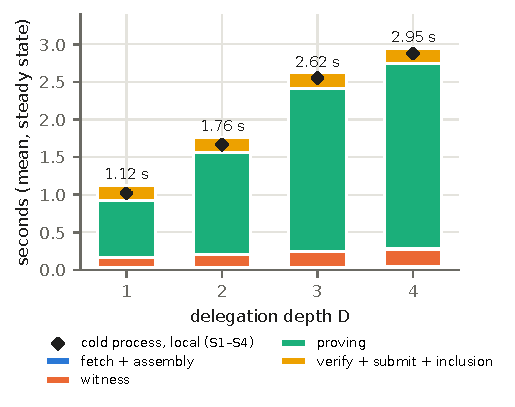
\includegraphics[width=\columnwidth]{figures/F1_latency_by_stage.pdf}
  \caption{Lifecycle latency of one fresh action by stage (mean of \NNSteady{} fresh actions per depth, steady state); diamonds: local
  computation in a fresh process. Proving dominates.}
  \label{fig:latency}
\end{figure}
\emph{Latency.} Fig.~\ref{fig:latency} breaks one fresh action into fetching paths, witness assembly and calculation, proving, off-chain
verification, submission and inclusion. The local authorization computation takes \NLocalA, \NLocalB, \NLocalC{} and \NLocalD\,s for $D=1..4$
(\NNSteady{} fresh actions per depth in three process blocks), of which proving takes \NProveA--\NProveD\,s; each hop adds \NSlopeHop\,ms
(95\,\% CI \NSlopeLo--\NSlopeHi). A cold process adds \NColdDeltaA--\NColdDeltaD\,ms to the action. All three pre-registered targets hold at
$D=4$: p95 local computation \NPninetyfiveSteady\,s (cold \NPninetyfiveCold\,s) $\le 10$\,s, peak memory \NPeakRss\,GiB $\le 8$\,GiB,
verifier-only gas \NVerifierGas{} $\le 500$k.

\begin{figure}[t]
  \centering
  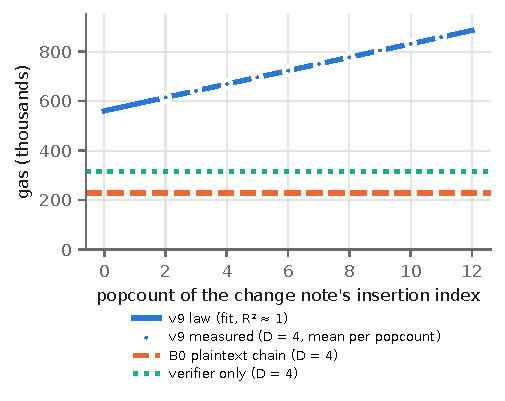
\includegraphics[width=\columnwidth]{figures/F2_gas_vs_note_index.pdf}
  \caption{Execute gas at $D=4$ against the number of one-bits of the change note's insertion index (\NWorldDfour{} actions), the fitted law, the
  plaintext lower bound B0 and the verifier alone.}
  \label{fig:gas}
\end{figure}
\emph{Gas.} The full transaction cost of an action is set by the note-tree insertion, not by the depth (Fig.~\ref{fig:gas}):
gas $=\text{\NLawBase} + \text{\NLawPop}\cdot\mathrm{popcount}(i) + \text{\NLawD}\cdot D$ ($R^2=\NLawRsq$), where $i$ is the insertion index of the change note.
An action costs \NGasVnineFreshD{} gas on an almost empty note tree and \NGasWorldD{} on average with \NNoteLeaves{} notes; a gas figure is
therefore only meaningful together with the note-tree size.

\emph{Scale.} \NWorldAgents{} agents (\NWorldDfour{} at depth~4) with budgets delegated by real transfer transactions acted concurrently on the same state:
\NEpochAcc/\NEpochOf{} actions were accepted in \NEpochBlocks{} blocks of 30M gas (\NEpochPerBlock{} per block). One machine produced
\NProofsPerMin{} proofs per minute.

\emph{Cost of privacy and of each component.} A plaintext implementation of the same policy in the same contract stack (B0: ECDSA certificate
chain, per-hop revocation, replay set, per-edge budget ledger) costs \NBzeroMedA--\NBzeroMedD{} gas for $D=1..4$; v9 costs
\NRatioFreshD--\NRatioFreshA$\times$ that on a fresh note tree and \NRatioWorldD--\NRatioWorldA$\times$ at the size of our world, with the ratio
falling as $D$ grows (the larger values at $D=1$). In proving time, accountability adds \NAcctCostD\,ms and budget notes add \NBudgetCostD\,ms at $D=4$
(Fig.~\ref{fig:components}); at $D=3$ accountability crosses a power-of-two FFT domain and adds \NAcctCostC\,ms.
\begin{figure}[t]
  \centering
  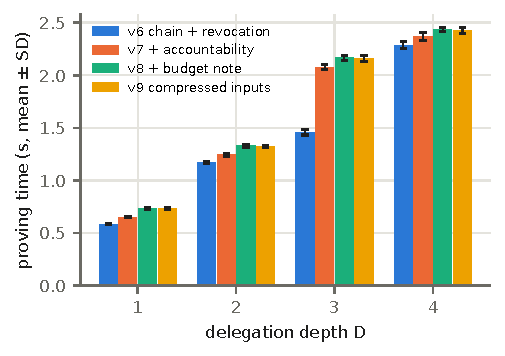
\includegraphics[width=\columnwidth]{figures/F3_component_cost.pdf}
  \caption{Proving time of successive circuit versions, \NNSteady{} fresh instances per cell (mean $\pm$ SD).}
  \label{fig:components}
\end{figure}

\subsection{Comparison with neighbouring systems}
\label{subsec:eval-baselines}
We ran the official implementations natively instead of excluding systems built on other stacks, and compared only sub-tasks they support.
UCAN (go-ucan) verifies a depth-4 delegation in \NUcanVerifyD\,ms with \NUcanBytesD\,bytes of tokens, with the lineage in clear and no revocation
in the implementation. The DAC scheme from equivalence-class signatures shows a credential in \NDacShowA\,ms and verifies it in \NDacVerifyA\,ms;
its code supports a single delegation level. zk-creds proves an expiry show in \NZkcMono\,ms (one witness, repeated) and has no delegation.
ZKM, ZK-ACE and ZEBRA have no public code and are compared at protocol level: ZKM shares hidden lineage, in-circuit conservation and on-chain
verification but revokes only whole subtrees and offers only voluntary disclosure; ZK-ACE has no delegation. These systems do not offer the same
functionality, so the timings are not a like-for-like comparison; what the comparison shows is the combination our system adds and its cost
relative to the plaintext bound above.

\subsection{Machine-checked invariants}
\label{subsec:eval-lean}
A Lean~4 model of the gate (mint, split, delegate, execute, revoke, time) proves, for every reachable state, budget conservation (unspent plus spent
equals minted), subtree conservation (below any certificate edge, spending never exceeds what was minted or delegated into it), monotonic
revocation and freezing (after the window nothing below a revoked edge is spent): \NLeanStmts{} theorem statements with \NLeanSorry{} uses of
\texttt{sorry} and only Lean's standard axioms. The model abstracts the cryptography by stated assumptions (knowledge soundness, commitment binding,
nullifier injectivity) and is checked for non-vacuity: removing the nullifier check lets the model spend twice its budget.

\subsection{Limitations}
\label{subsec:eval-limits}
One machine and one prover (snarkjs); native provers were not tested. The chain is a local anvil node, so inclusion latency excludes block time
and finality. Phase~2 of the setup is not a ceremony. Tree heights are fixed by the compiled circuits and were not swept; depths beyond 4 were not
compiled. The anonymity of v9 transcripts was not tested empirically, and the anonymity and no-false-framing arguments remain paper proofs.
